\section{Product perspective}
\textit{MyTaxyService} will not be integrated with any other systems, it will be self-contained.\\
It will be implemented in a three-tier architecture. Server-side, on the application layer there will be the Queue Manager (will take care of managing taxi queues in the various zones) and the Reservation System (will allow taxis to be reserved in advance). A dedicated server will host the database in which the system will store all the data.\\
Passengers will be able to access the system after a registration and a following login from both a web application and a mobile application (available for free for the three major mobile operating systems, Android, IOS, Windows Phone from their markets).\\
Taxi drivers instead, will use a different version of the application that will not be available on the markets but will be provided by the government upon a request.

\begin{figure}[h]
	\centering
	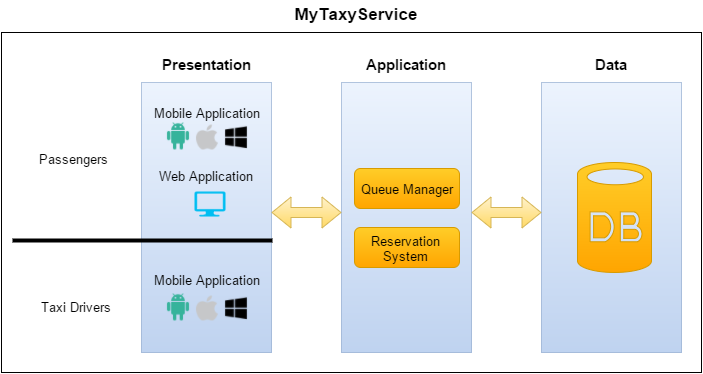
\includegraphics[width=4in]{Images/system_diagram}
	\caption{Schematic representation of \textit{MyTaxyService}}
\end{figure}